\subsection{Screen}

The Screen class is used to map the Game onto the Display. This is to keep all the drawing calculation the same place.

The Area's representation only knows about Fields, and which are next to each other. This class maps this info unto the Screen. Therefore the game only knows which fields are next to each other, and not how they are displayed on the screen.

\subsubsection{Layout}

The first revision was simply to map each field to a 3-by-3 square (see~\ref{fig:screen_fields_rev1}) which worked, but it became really hard to visualize how the snake was tangled as it often was represented like a black blob (see Figure~\ref{fig:screen_fields_rev1}). 

In the next revision, we added a border to the fields, which was easy to do, as all the drawing and calculations was already collected in this class. This change meant that each field shares it's borders with the neighbor field. So that when the snake head is drawn, it is not allowed to draw in the border, as it does not know from where it came (see the yellow marking in Figure~\ref{fig:screen_fields_rev2}). The same applies to the part before. It knows only that it goes to the right, and therefore fills out the right border (see the red marking in Figure~\ref{fig:screen_fields_rev2}), but are not allowed to touch the other borders, as it also doesn't know where it came from.

\begin{figure}
\centering
\begin{minipage}{.5\textwidth}
  \centering
	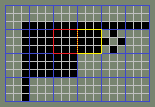
\includegraphics[width=.9\textwidth]{implementation/screen_fields_rev1}
	\caption{First Revision Display Layout}
	\label{fig:screen_fields_rev1}
\end{minipage}%
\begin{minipage}{.5\textwidth}
  \centering
	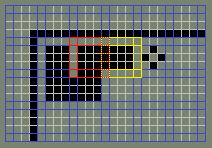
\includegraphics[width=.9\textwidth]{implementation/screen_fields_rev2}
	\caption{Second Revision Display Layout}
	\label{fig:screen_fields_rev2}
\end{minipage}
\end{figure}

The most important method in the screen class is the \texttt{convert\_point} (see Listing~\ref{lst:convert_point}), as this does the mapping between the two representations of the Area. It return the Point that matches the upper left corner of the 3-by-3 Field.

\begin{lstlisting}[caption={Converting an Area's point to a Display's point},label={lst:convert_point},frame=tlrb, language=C++]{Name}
buffer_point_type convert_point(const point_type& point) const {
    return buffer_point_type{point.x * 4 - 2, point.y * 4 - 2};
}
\end{lstlisting}

The offsetting is made to squeeze in an extra Field, as the border only need a single pixel to be drawn. So if the border would be changed to actually fill the 3-by-3, it wouldn't be displayed on the Display.

\subsubsection{Drawing objects}

To draw the Snake going right, it simply draws a rectangle based on the buffer point, it is given (see Listing~\ref{lst:draw_snake}).

\begin{lstlisting}[caption={Drawing a snake turning right},label={lst:draw_snake},frame=tlrb, language=C++]{Name}
// Example Implementation
void draw_snake_right(const point_type& point) {
  auto buffer_point = convert_point(point);
  buffer_->draw_square(buffer_point, 4 , 3);
}
\end{lstlisting}

\subsubsection{Drawing text}

To enable the use of text without to much calculations, we use a font that is 8 pixels high and uses a \texttt{uint8\_t} rows as lines. We can then use the ScreenBuffer's \texttt{set\_data} function to write directly in the buffer.

To keep the sprites of the alphabet, we use a large array with the ASCII chars from 0 to Z and space. So to draw a char, we calculate the correct place (see Listing~\ref{lst:sprite_location}) in the array and read out the sprite data for that single char, and sends it to the ScreenBuffer (see Listing~\ref{lst:draw_char})

\noindent\begin{minipage}[t]{.45\textwidth}
\begin{lstlisting}[caption={Drawing a Char},label={lst:draw_char},frame=tlrb, language=C++]{Name}
array_point_type WriteChar(array_point_type array_point, const char& letter){

    // Write the Char Sprite
    for (auto itr = TextEncoding::begin(letter); itr != TextEncoding::end(letter); --itr) {
  	   buffer_->set_data(array_point, *itr);
  		 ++array_point.column;
  	}

    // Write a "space" after a character, this is to save space in the TextData array
    buffer_->set_data(array_point, 0x00);
  	++array_point.column;

    // Return the next position for the next Char
  	return array_point;
}
\end{lstlisting}
\end{minipage}\hfill
\begin{minipage}[t]{.45\textwidth}
\begin{lstlisting}[caption={Calculating Sprite Location},label={lst:sprite_location},frame=tlrb, language=C++]{Name}
static const uint8_t* begin(unsigned char ch) {
    // Move ' ' as it's not near they others in ascii value
    ch = (ch == ' ' ? 'Z' + 1 : ch);
    return &TextData[((ch - '0')*5)+4];
}

static const uint8_t* end(unsigned char ch) {
    // All out sprites has a width of 5
    return begin(ch) - 5;
}
\end{lstlisting}
\end{minipage}

As we now can draw a single char, it's easy to draw a string via a loop, and a number via the \texttt{itoa} method.
